% ----------------------------------------------------------
\chapter{Testes de Gráficos}
\label{cha:testesgraficos}
\index{Testes de Gráficos}
% ----------------------------------------------------------

Este apêndice reúne, para fins de verificação visual, os diagramas UML e PlantUML
produzidos ao longo da modernização do sistema — desde a base algorítmica em Java
(Desktop) até a reescrita final em Python/Streamlit. Cada diagrama é apresentado em
uma figura individual, identificada por seção e \textit{label} próprios para permitir
referência cruzada em seções posteriores.

\section{Diagrama de Arquitetura em Camadas --- Java e Python}
\label{sec:diagarquitetura}

Complementando os diagramas de classes, atividade e sequência das seções
seguintes, as Figuras~\ref{fig:arquitetura_java} e~\ref{fig:arquitetura_python}
apresentam a organização em camadas de cada sistema, permitindo comparar
diretamente como a mesma separação de responsabilidades (interface,
orquestração/controle e núcleo algorítmico) foi realizada em cada plataforma.

\begin{figure}[H]
    \caption{Arquitetura em camadas --- Sistema legado (Java Desktop)}
    \centering
    \begin{tikzpicture}[
        layer/.style={draw, rounded corners, minimum width=8cm,
                      minimum height=1.2cm, align=center, fill=#1},
        arrow/.style={-{Stealth}, thick}
    ]
        \node[layer=blue!15] (view) {Camada de Apresentação\\\texttt{Swing/AWT} (\texttt{JFrame}, \texttt{JPanel}, \textit{listeners})};
        \node[layer=green!15, below=0.8cm of view] (controller) {Camada de Controle\\Orquestração de eventos (\texttt{ActionListener})};
        \node[layer=orange!15, below=0.8cm of controller] (model) {Núcleo Algorítmico\\\texttt{BaggingOptimized.java} + EJML (\texttt{SimpleMatrix})};

        \draw[arrow] (view) -- (controller);
        \draw[arrow] (controller) -- (model);
    \end{tikzpicture}
    \caption*{Fonte: \oautor}
    \label{fig:arquitetura_java}
\end{figure}

\begin{figure}[H]
    \caption{Arquitetura em camadas --- Sistema modernizado (Python/Streamlit)}
    \centering
    \begin{tikzpicture}[
        layer/.style={draw, rounded corners, minimum width=8cm,
                      minimum height=1.2cm, align=center, fill=#1},
        arrow/.style={-{Stealth}, thick}
    ]
        \node[layer=blue!15] (apresentacao) {Camada de Apresentação\\\texttt{app.py} --- Streamlit (orquestração de UI e sessão)};
        \node[layer=green!15, below=0.8cm of apresentacao] (visual) {Camada de Visualização\\\texttt{components.py} --- Plotly (fábrica de gráficos)};
        \node[layer=orange!15, below=0.8cm of visual] (nucleo) {Núcleo Algorítmico\\\texttt{models.py} --- NumPy (\texttt{np.linalg.lstsq})};

        \draw[arrow] (apresentacao) -- (visual);
        \draw[arrow] (visual) -- (nucleo);
    \end{tikzpicture}
    \caption*{Fonte: \oautor}
    \label{fig:arquitetura_python}
\end{figure}

Observa-se que a camada de núcleo algorítmico, isolada de qualquer dependência
de interface em ambos os sistemas, é justamente onde reside a lógica validada
pelos testes de paridade amostra-a-amostra (Apêndice~\ref{cha:paridadeamostra})
e pelos testes de caixa-preta (Seção~\ref{sec:testescaixapreta}).

\section{Diagrama de Classes --- Java}
\label{sec:diagclassejava}

\begin{figure}[htbp]
	\caption{Diagrama de classes.}
	\centering
		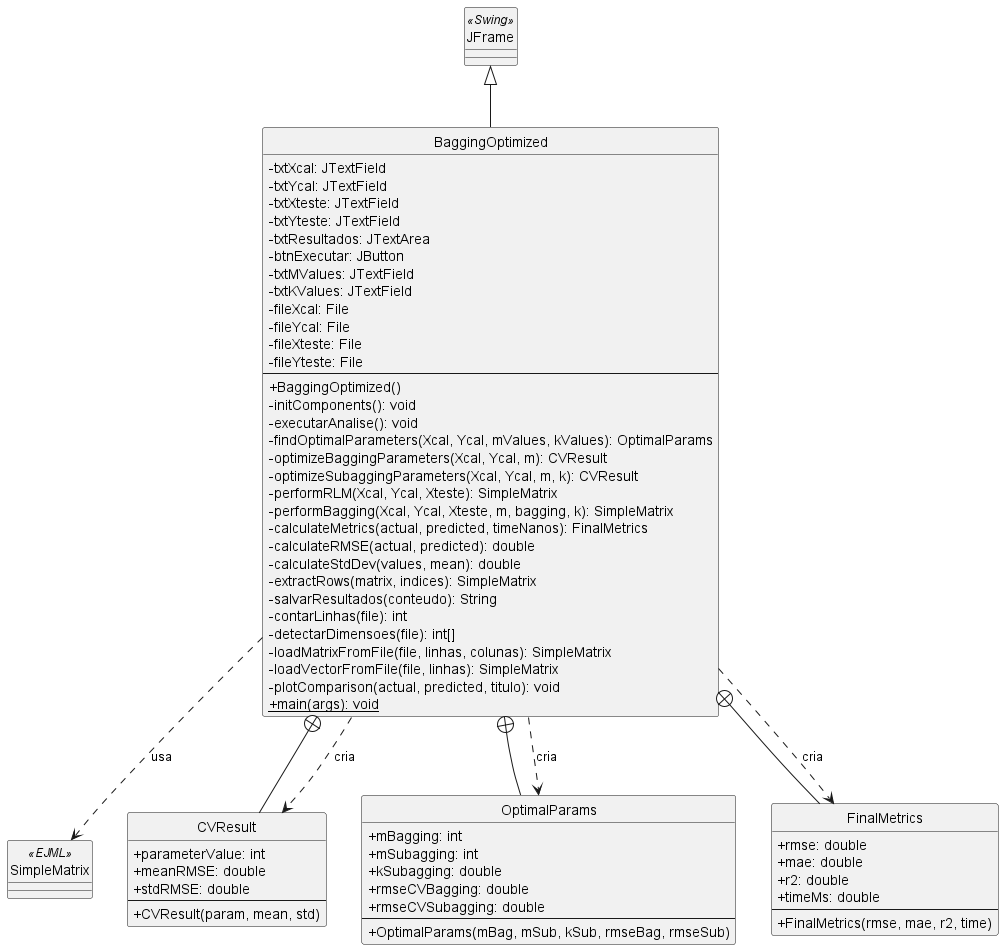
\includegraphics[width=1.00\textwidth]{./outros/fig/E_Diagramas/out/diag_classe/BaggingOptimized_Classe.png}
	\caption*{Fonte: \oautor}
	\label{fig:BaggingOptimized_Classe}
\end{figure}

\newpage
\section{Diagrama de Atividade --- Java}
\label{sec:diagatividadejava}

\begin{figure}[htbp]
	\caption{Diagrama de atividades.}
	\centering
		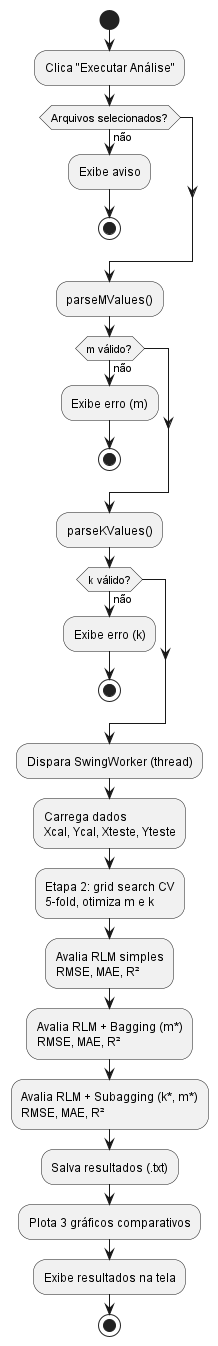
\includegraphics[width=0.20\textwidth]{./outros/fig/E_Diagramas/out/diag_sequencia/BaggingOptimized_Atividade.png}
	\caption*{Fonte: \oautor}
	\label{fig:BaggingOptimized_atividades}
\end{figure}

\newpage
\section{Diagrama de Sequência --- Java}
\label{sec:diagsequenciajava}

\begin{figure}[htbp]
	\caption{Diagrama de sequência.}
	\centering
		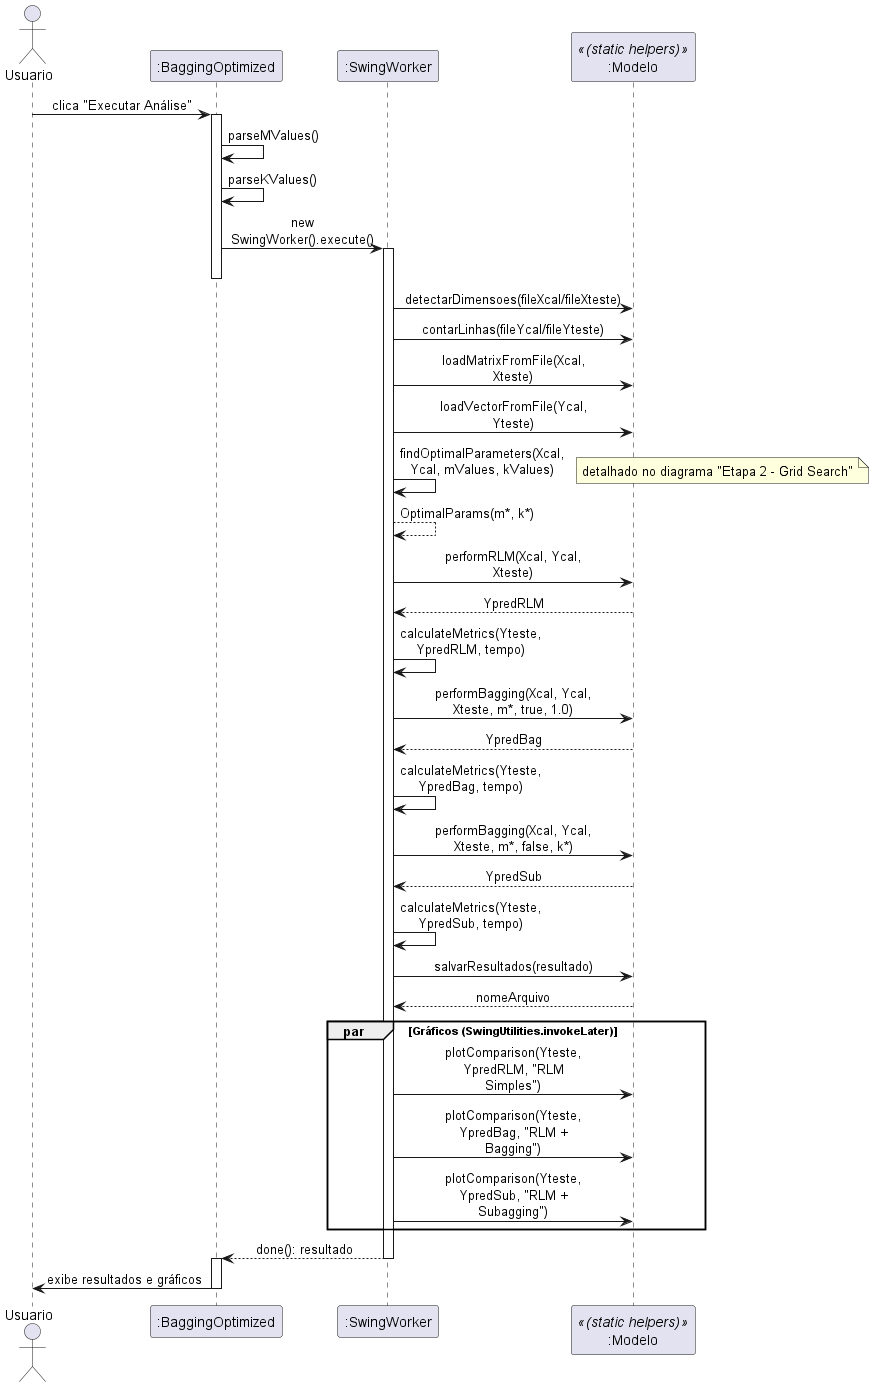
\includegraphics[width=0.75\textwidth]{./outros/fig/E_Diagramas/out/diagrama/BaggingOptimized_FluxoCompleto.png}
	\caption*{Fonte: \oautor}
	\label{fig:BaggingOptimized_sequencias}
\end{figure}

\newpage
\section{Diagrama de Atividades --- Java (PlantUML)}
\label{sec:diagatividadejavaplantuml}

\begin{figure}[htbp]
	\caption{Diagrama de atividade PlantUML.}
	\centering
		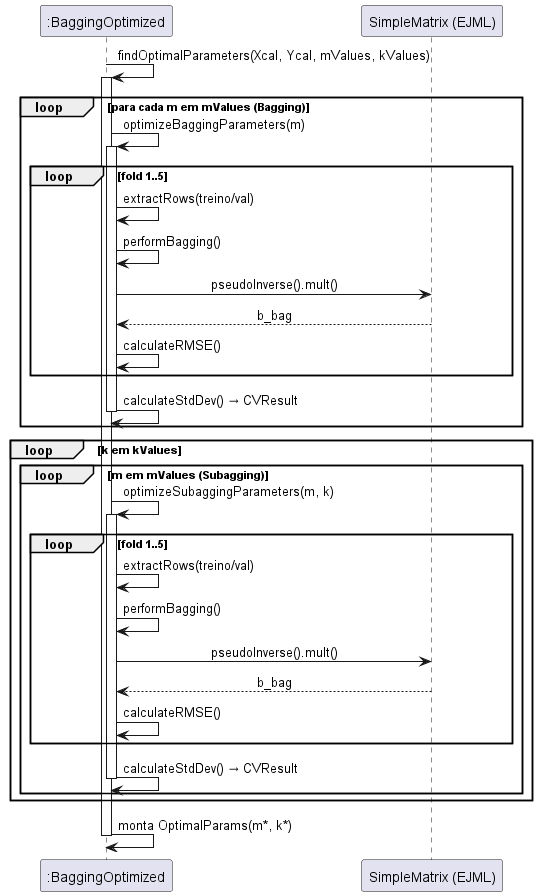
\includegraphics[width=0.50\textwidth]{./outros/fig/E_Diagramas/out/diagrama02/Etapa2_GridSearch_CV.png}
	\caption*{Fonte: \oautor}
	\label{fig:BaggingOptimized_atividade}
\end{figure}

\newpage
\section{Diagrama de Atividades --- Streamlit}
\label{sec:diagatividadestreamlit}

\begin{figure}[htbp]
	\caption{Diagrama de atividade PlantUML.}
	\centering
		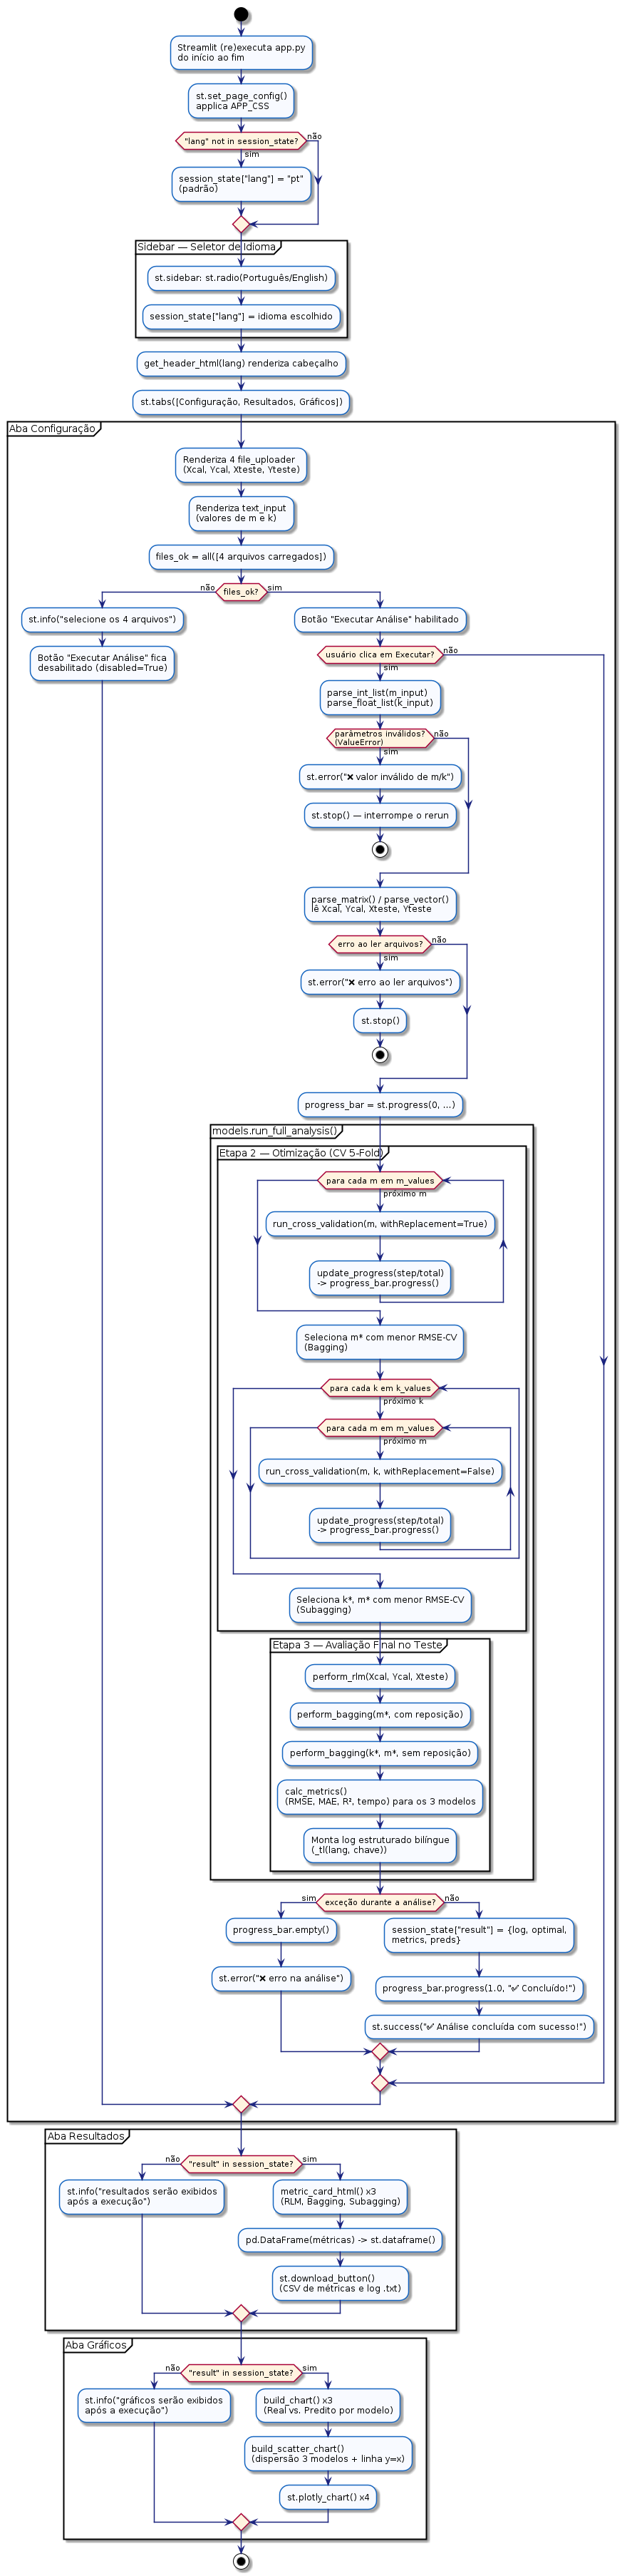
\includegraphics[width=0.30\textwidth]{./outros/fig/E_Diagramas/streamlit/diagrama_atividades_streamlit.png}
	\caption*{Fonte: \oautor}
	\label{fig:BaggingOptimized_atividade2}
\end{figure}

\newpage
\section{Diagrama de Classes (Módulos) --- Streamlit}
\label{sec:diagclassesstreamlit}

\begin{figure}[htbp]
	\caption{Diagrama de classes (módulos) PlantUML.}
	\centering
		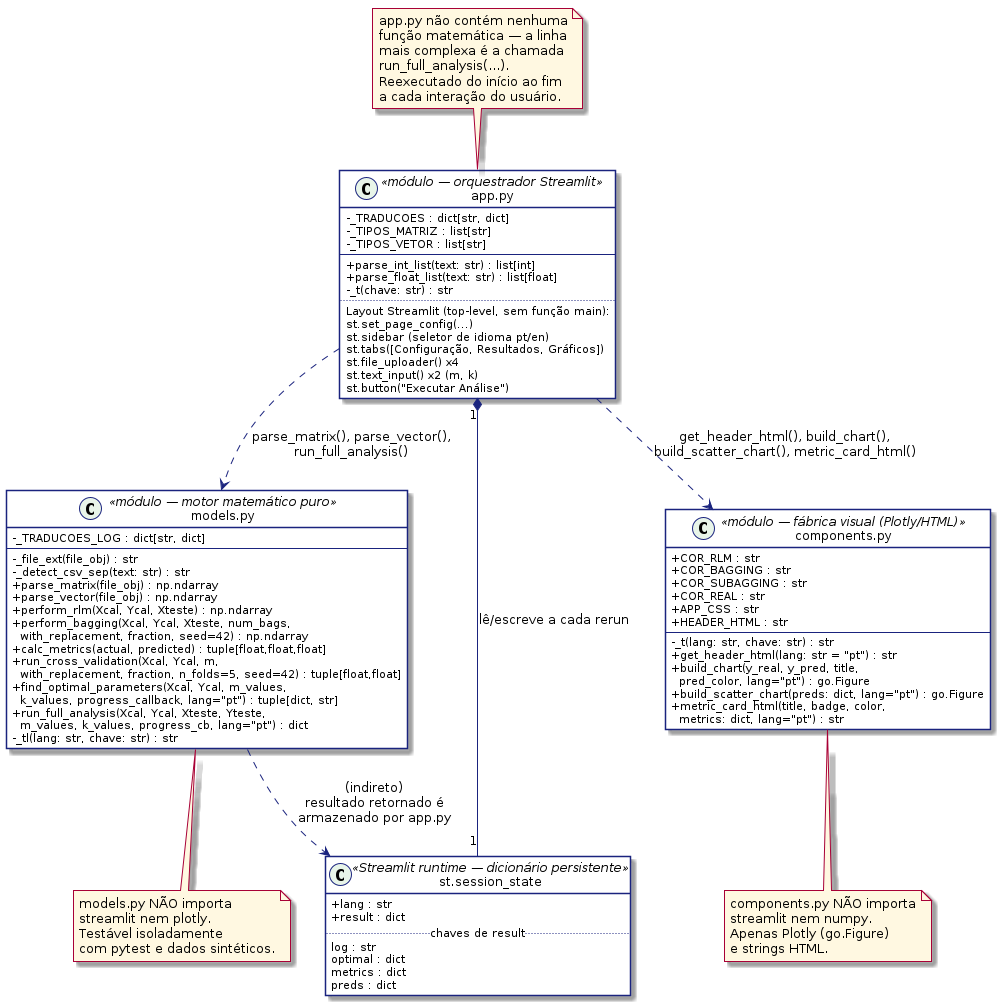
\includegraphics[width=0.85\textwidth]{./outros/fig/E_Diagramas/streamlit/diagrama_classes_streamlit.png}
	\caption*{Fonte: \oautor}
	\label{fig:BaggingOptimized_classe3}
\end{figure}

\newpage
\section{Diagrama de Sequência --- Streamlit}
\label{sec:diagsequenciastreamlit}

\begin{figure}[htbp]
	\caption{Diagrama de sequência PlantUML.}
	\centering
		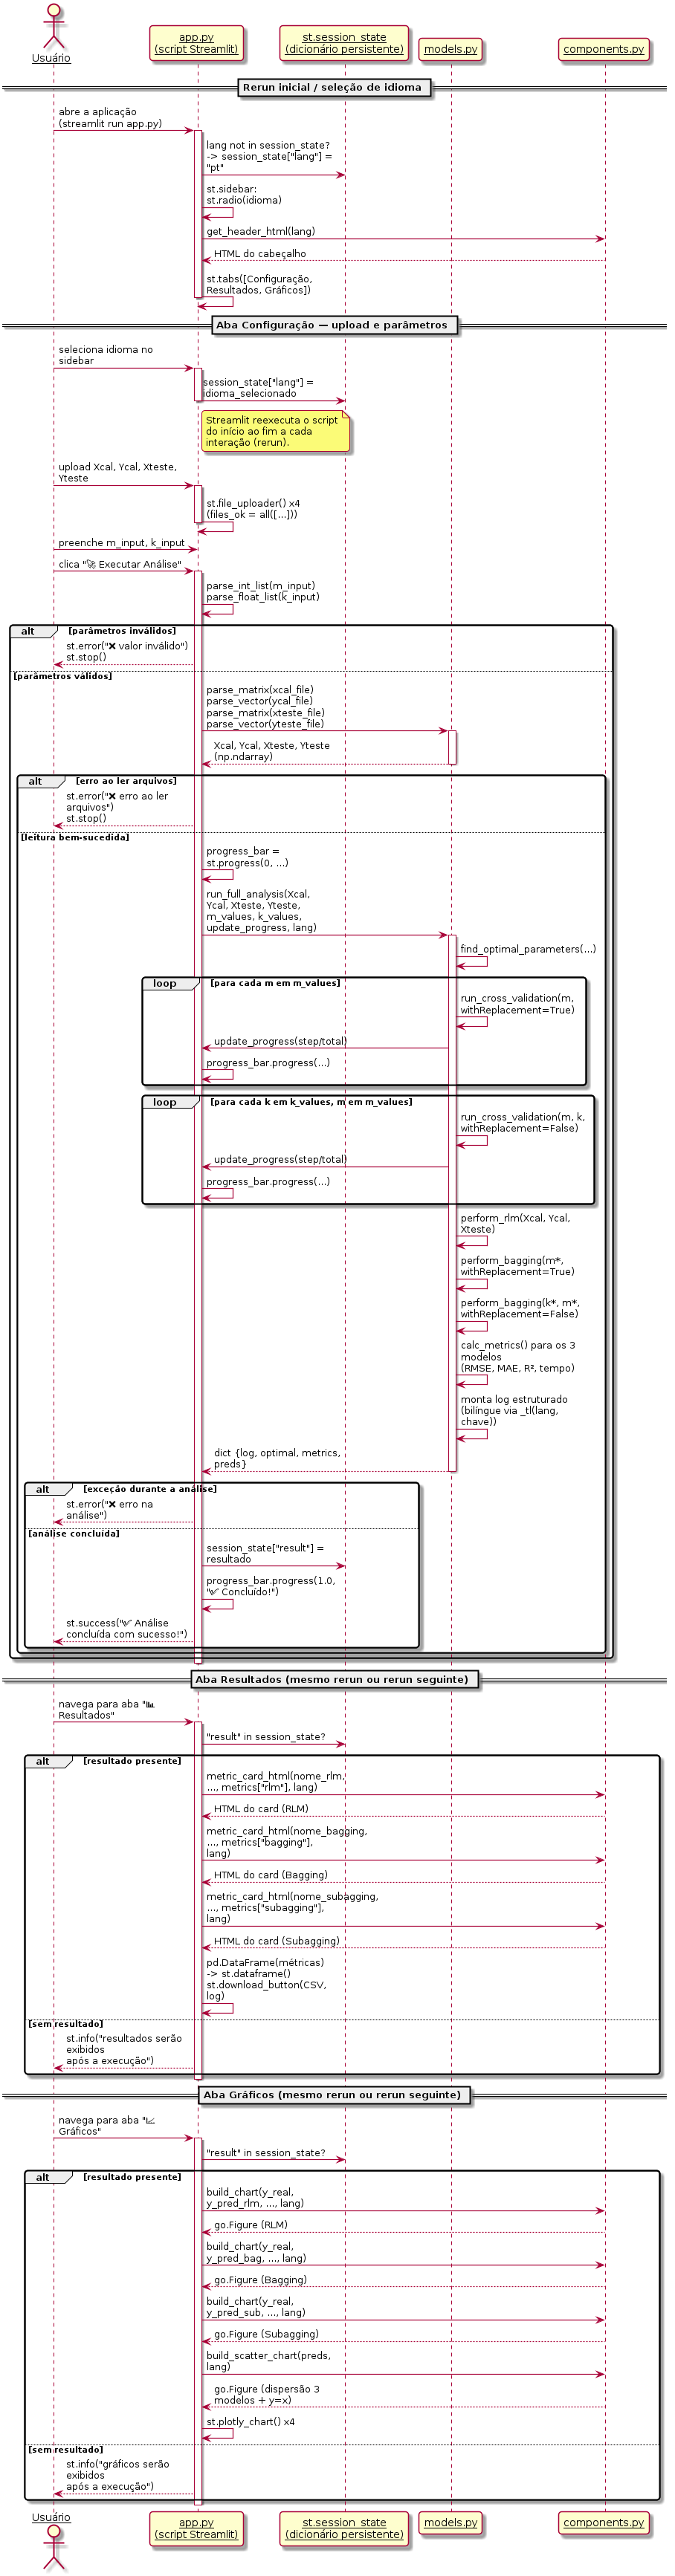
\includegraphics[width=0.30\textwidth]{./outros/fig/E_Diagramas/streamlit/diagrama_sequencia_streamlit.png}
	\caption*{Fonte: \oautor}
	\label{fig:BaggingOptimized_sequencia2}
\end{figure}